\section{Үр дүн}

Дээрх хэрэгжүүлэлтийн үр дүнд дараах зургуудад харагдаж байгаачлан манай веб апп маань ашиглахад бэлэн болсон. Доор гол гэсэн хуудсуудын ажиллаж буй процессыг илэрхийлэх хуудсуудын зургуудуудыг оруулав.
\clearpage


Хэрэглэгчийг угтан авах анхны нүүр хуудас. /тоглох, ранк, тухай навигацийг багтаасан болно./
\begin{figure}[h]
	\centering
	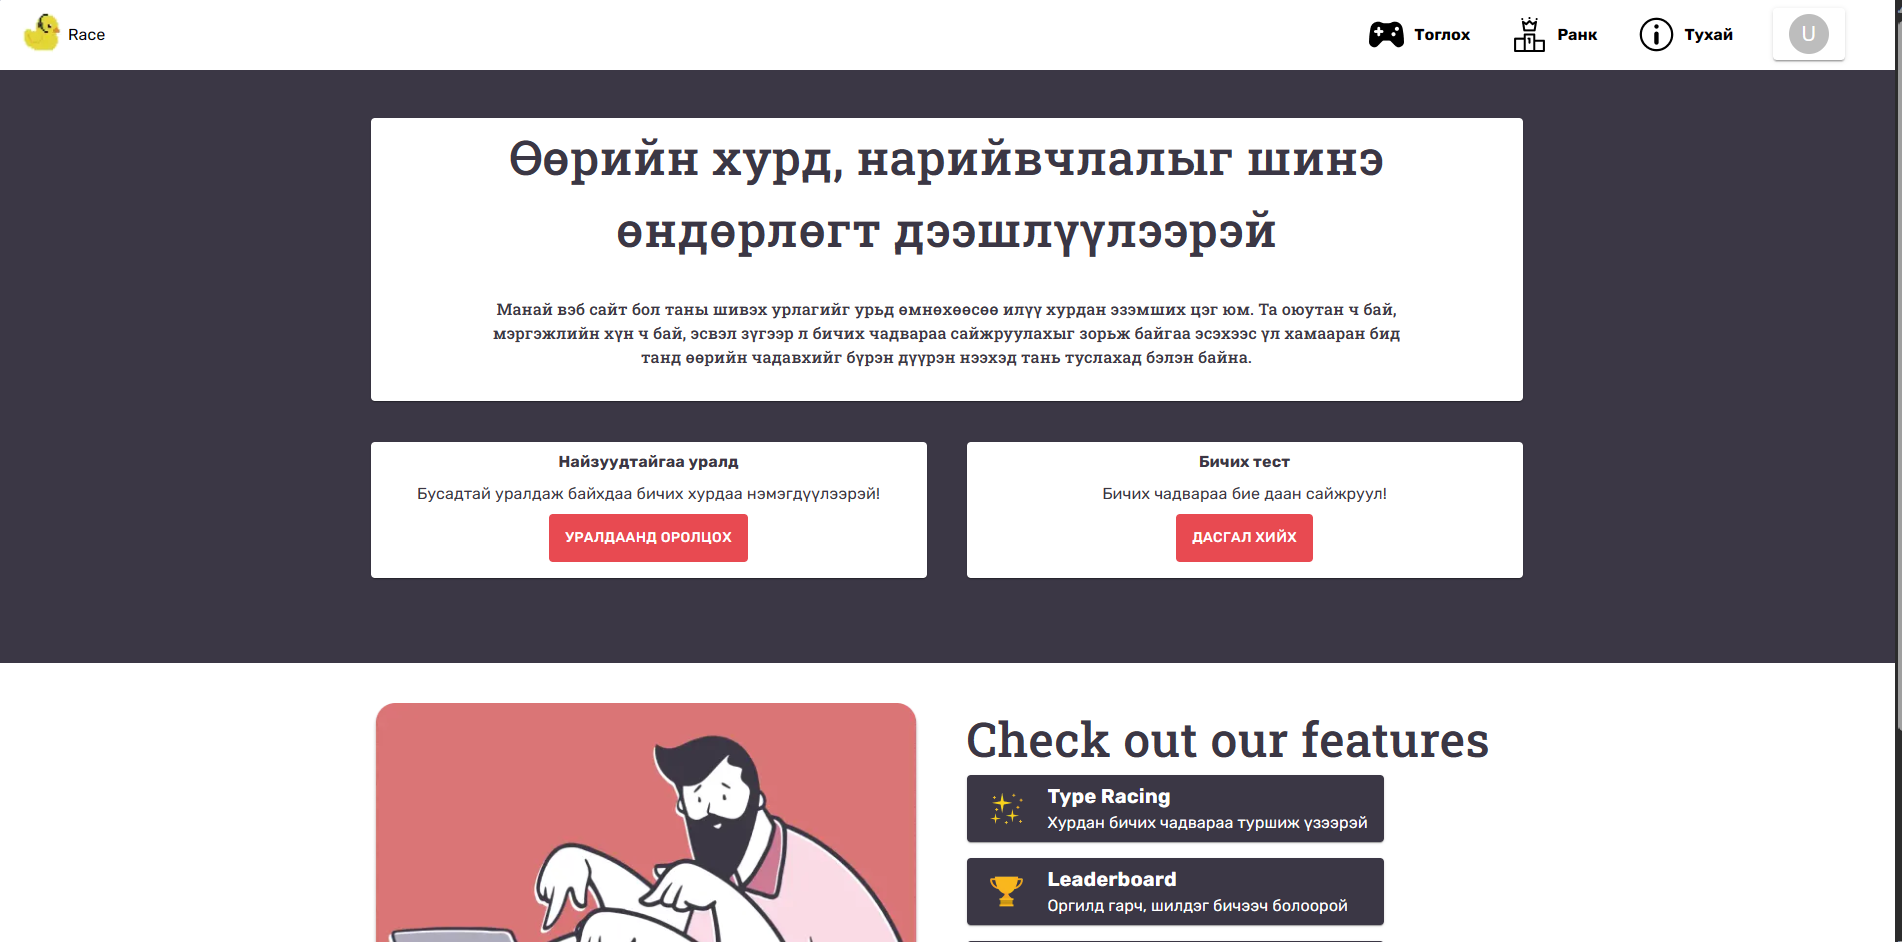
\includegraphics[width=13cm]{images/result/homepage.png}
	\caption{Нүүр хуудас}
	\label{fig:results}``''
\end{figure}

Singleplayer буюу зөвхөн өөрөө тест өгөх хуудас
\begin{figure}[h]
	\centering
	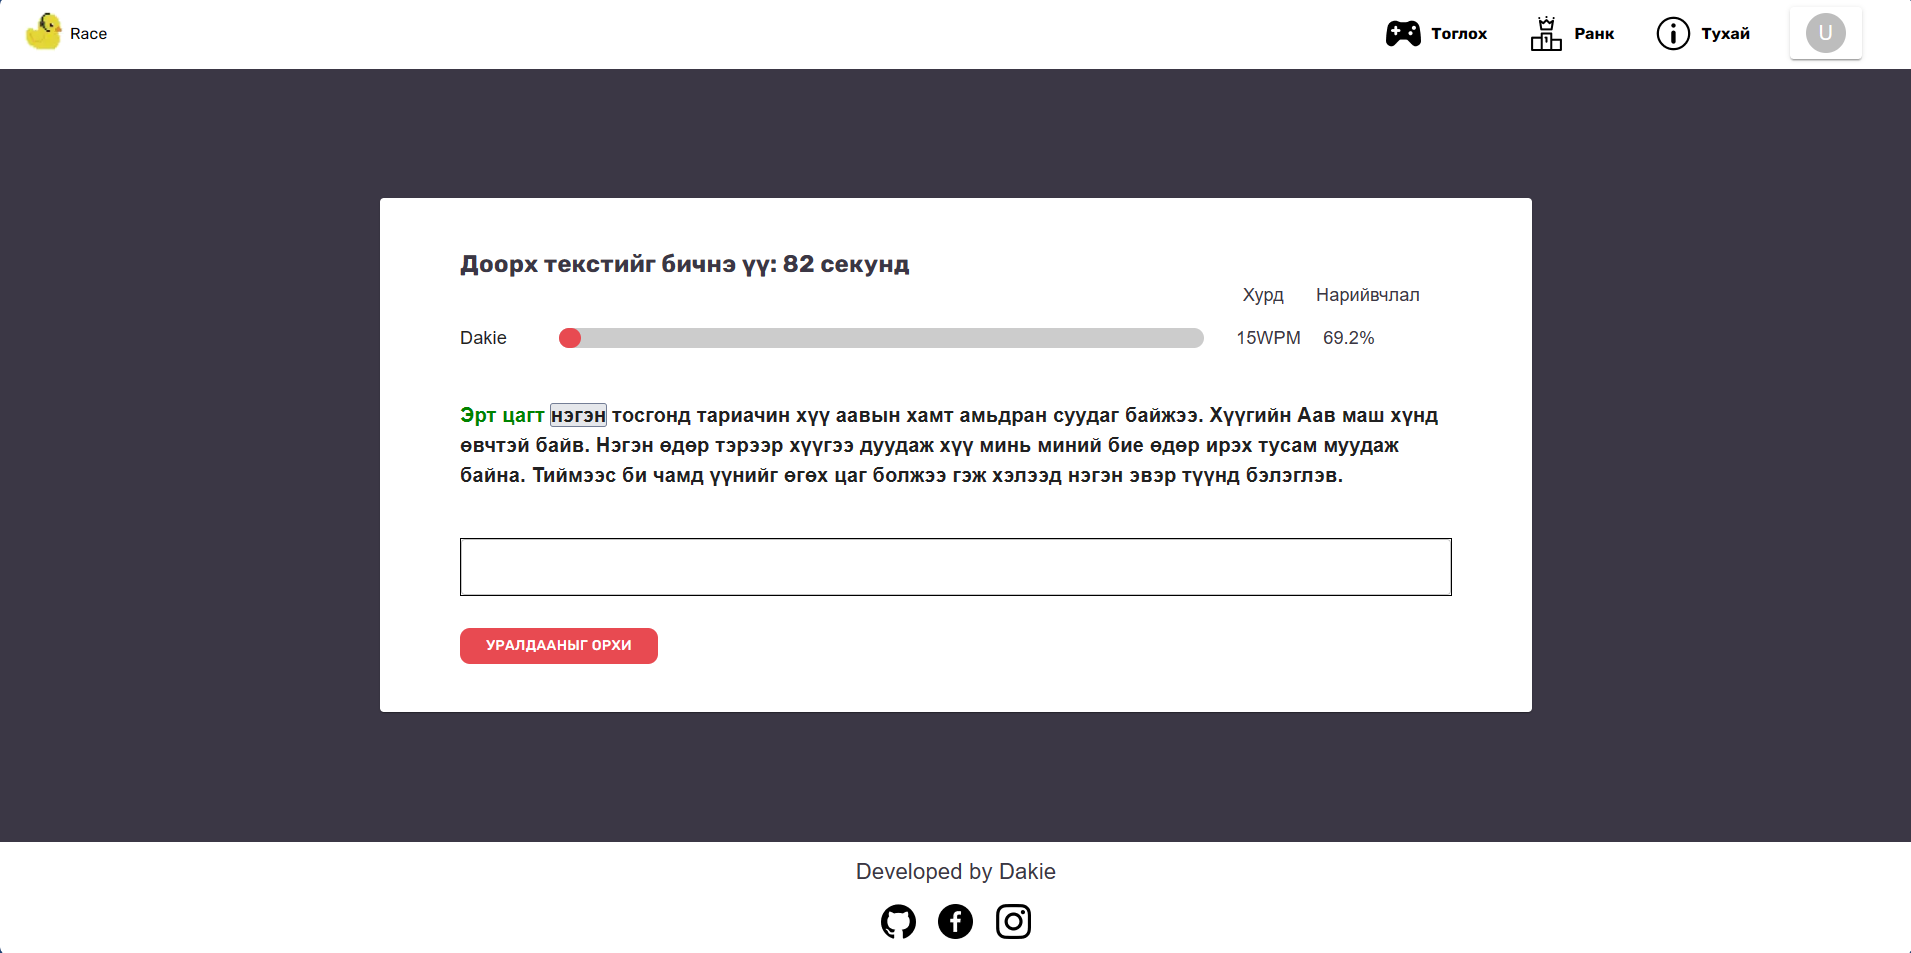
\includegraphics[width=13cm]{images/result/playpage.png}
	\caption{Хэрэглэгч шивэх тест өгөх хуудас}
	\label{fig:results}
\end{figure}

\clearpage
Нийт хэрэглэгчдийг үзүүлэлтээр нь эрэмбэлж харуулах хуудас. Мэдээллүүддийг 7 хоног, сар, жилээр филтэр хийн харах боломжтой.
\begin{figure}[h]
	\centering
	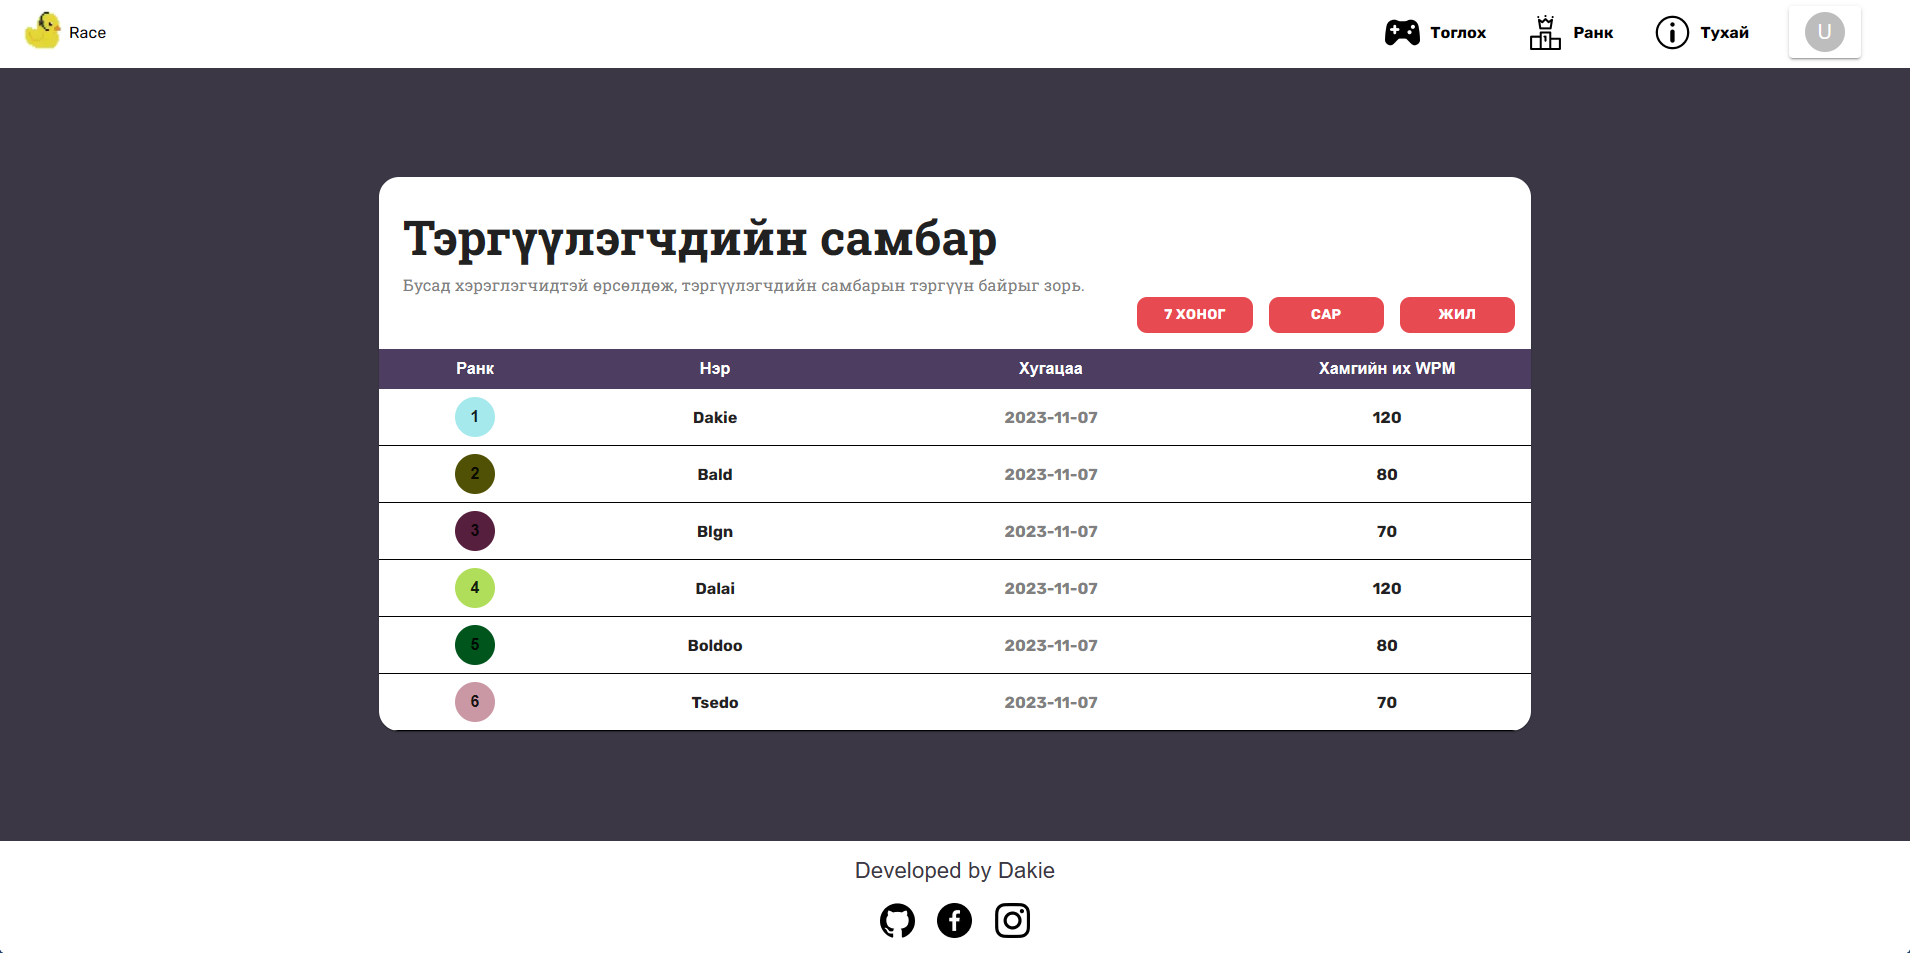
\includegraphics[width=13cm]{images/result/rankpage.png}
	\caption{Нийт тоглогчдыг тэргүүлэгчдийн хуудас}
	\label{fig:results}
\end{figure}

Хэрэглэгч хэрэв шивэх дасгалуудийг амжилттай хийн дуусгасан бол өөрийн үзүүлэлтүүдийг харах хуудас. /JSON ирж буй датануудыг filter хийх/ 
\begin{figure}[h]
	\centering
	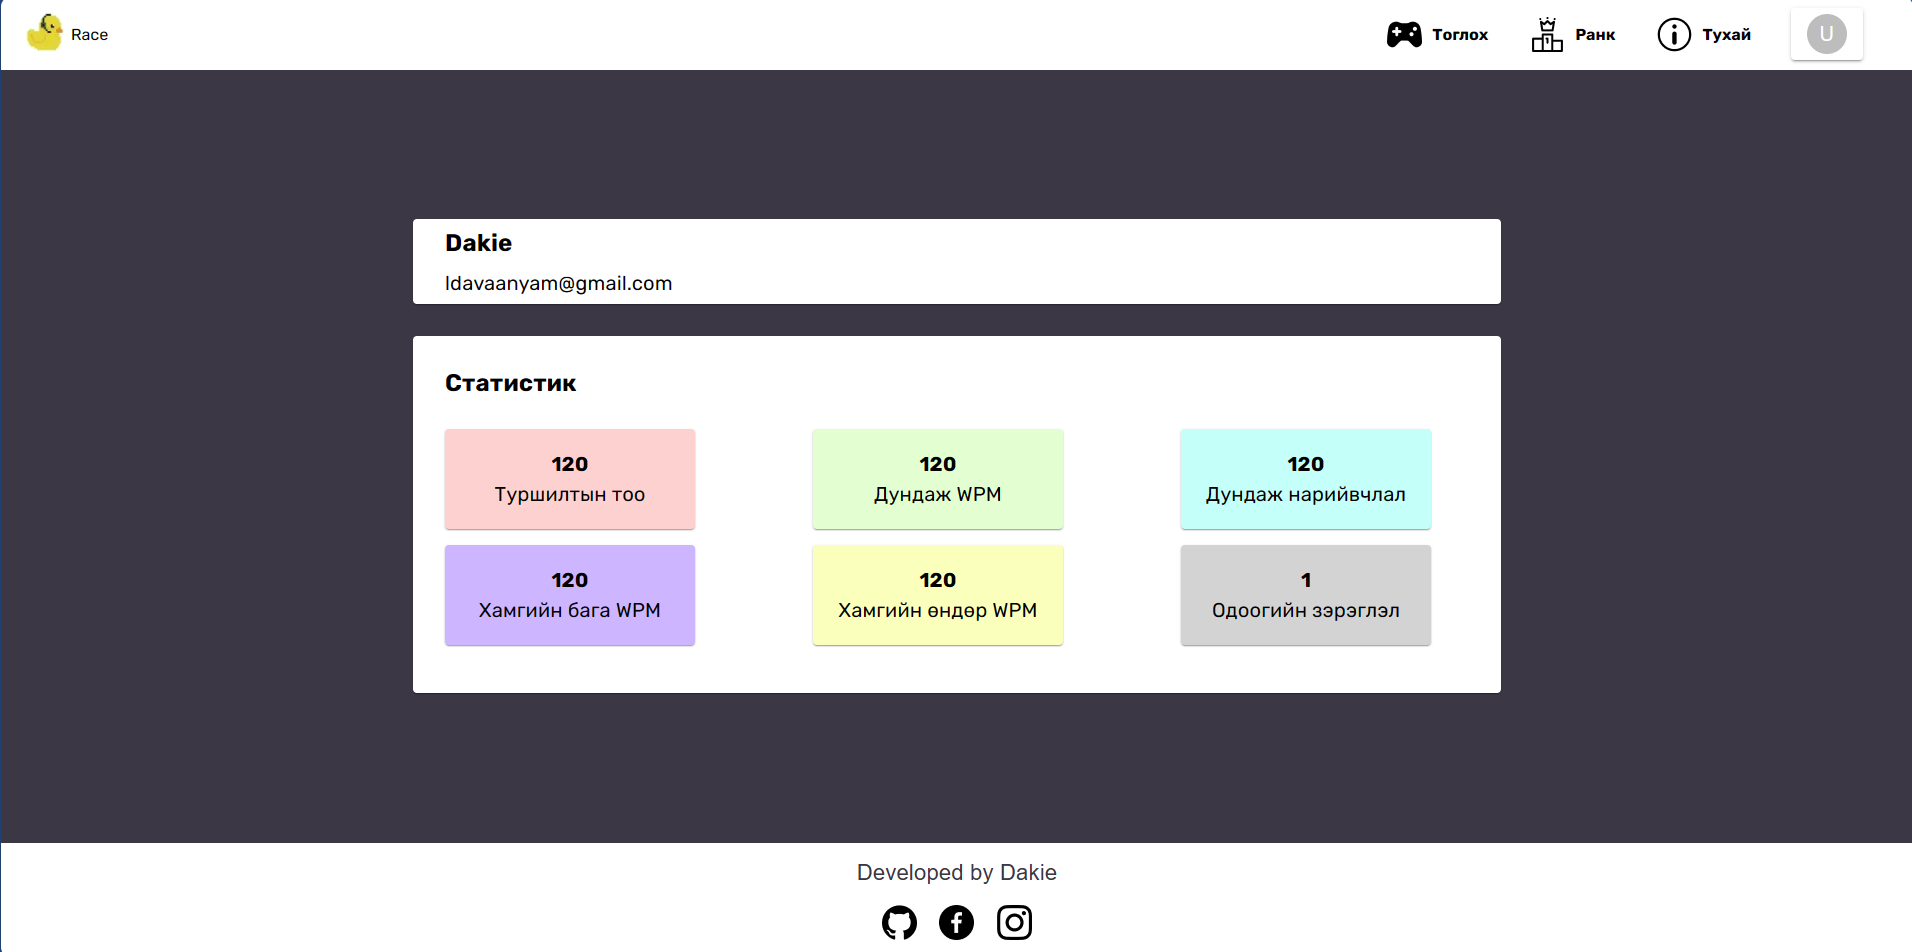
\includegraphics[width=13cm]{images/result/statisticspage.png}
	\caption{Хэрэглэгчийн статистикийн хуудас}
	\label{fig:results}
\end{figure}

\clearpage
Хэрэв хэрэглэгч нэвтрээгүй тохиолдолд рендер хийгдэх хуудас. Хэрэв бүртгэлгүй бол өөрийн майл болон нууц үгээ ашиглан нэвтрэх боломжтой.
\begin{figure}[h]
	\centering
	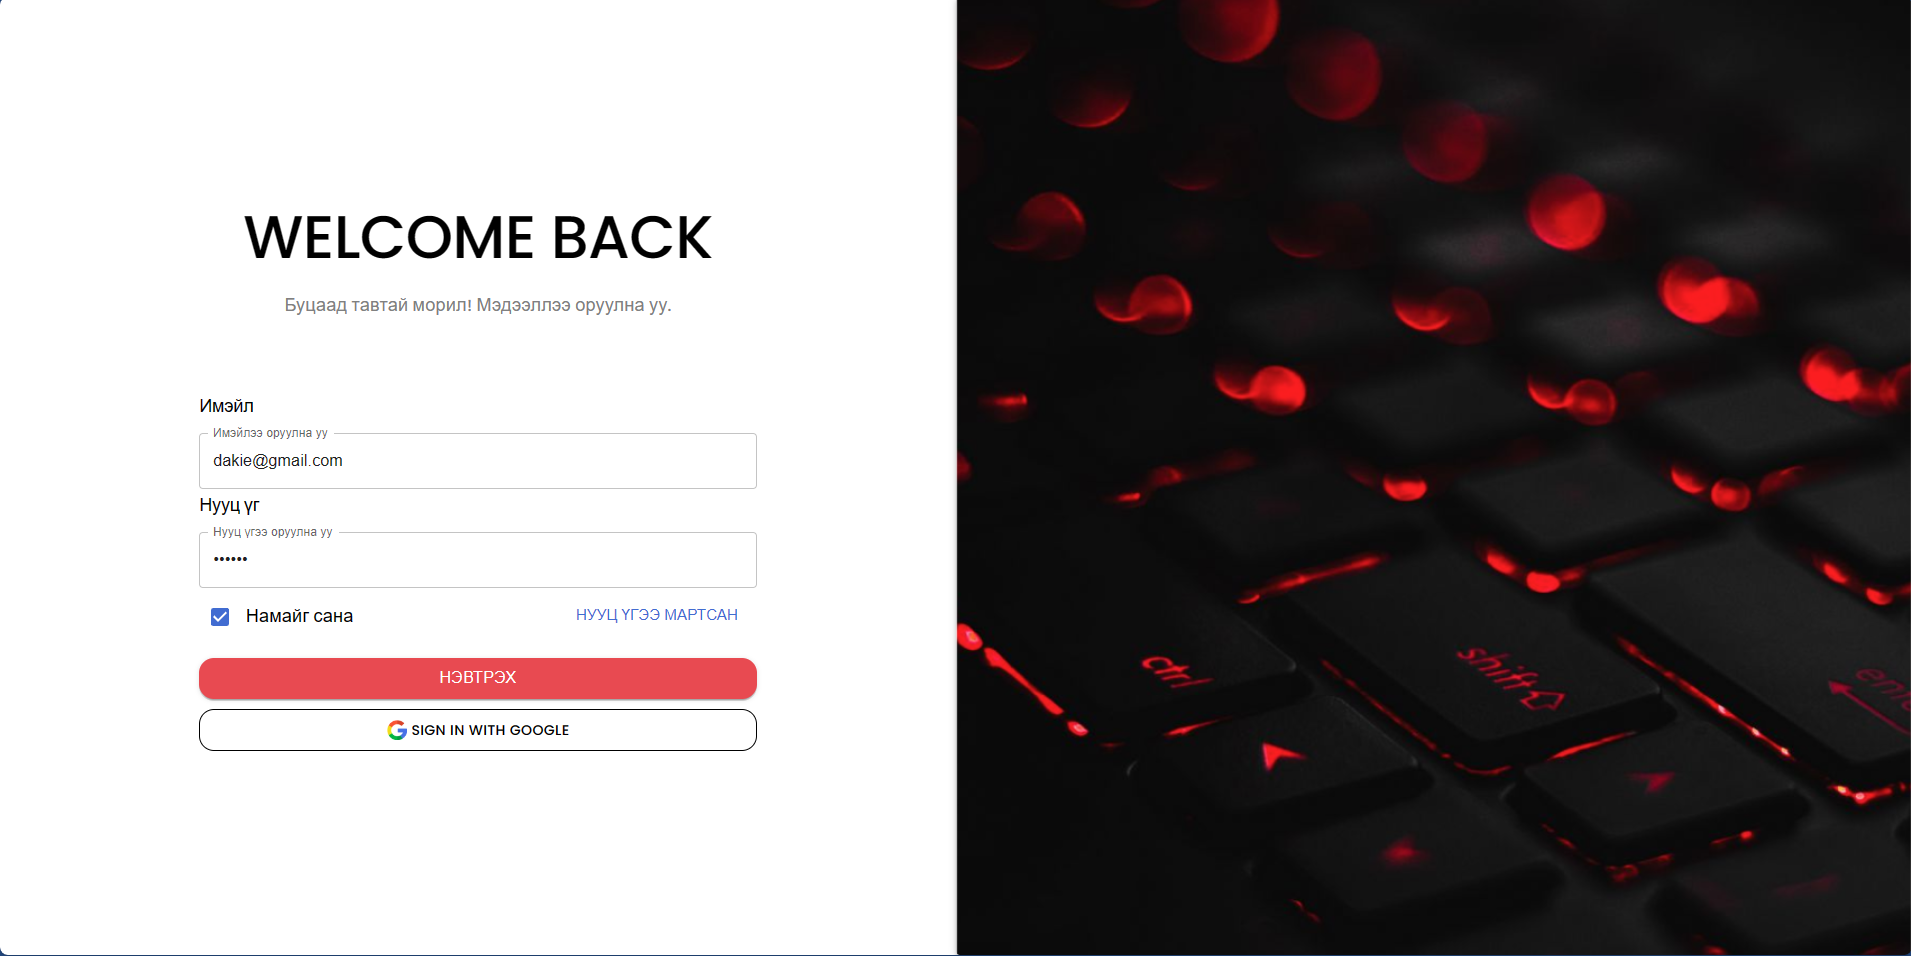
\includegraphics[width=13cm]{images/result/loginpage.png}
	\caption{Нэвтрэх хуудас}
	\label{fig:results}
\end{figure}